\documentclass{article}

\usepackage[utf8]{inputenc}
\usepackage[T1]{fontenc}
\usepackage{amsmath, amssymb, amsfonts}
\usepackage{graphicx}
\usepackage{hyperref}
\usepackage{booktabs}
\usepackage{float}
\usepackage{caption}
\usepackage{subcaption}
\usepackage{url}
\usepackage{color}
\usepackage{geometry}
\geometry{margin=1in}

\usepackage[numbers]{natbib}

\title{Understanding Hidden Computations in Chain-of-Thought Reasoning}

\author{Aryasomayajula Ram Bharadwaj \\
Independent Researcher \\
\texttt{ram.bharadwaj.arya@gmail.com}}

\date{}

\begin{document}

\maketitle

\begin{abstract}
Chain-of-Thought (CoT) prompting has significantly enhanced the reasoning abilities of large language models. However, recent studies have shown that models can still perform complex reasoning tasks even when the CoT is replaced with filler characters (e.g., ``\ldots''), leaving open questions about how models internally process and represent reasoning steps. In this paper, we investigate methods to decode these hidden computations in transformer models trained with filler CoT sequences. By analyzing layer-wise representations using the logit lens method and examining token rankings, we demonstrate that the hidden computations can be recovered without loss of performance. Our findings provide insights into the internal mechanisms of transformer models and open avenues for improving interpretability and transparency in language model reasoning.
\end{abstract}

\section{Introduction}

Chain-of-Thought (CoT) prompting has emerged as a powerful technique for improving the performance of large language models (LLMs) on complex reasoning tasks \cite{wei2022chain}. By encouraging models to generate intermediate reasoning steps, CoT prompting enables models to tackle problems that require multi-step reasoning. However, recent work by \cite{pfau2023let} demonstrates that these improvements can be achieved even when the CoT is replaced with hidden or filler characters (e.g., ``\ldots''). This raises intriguing questions about the nature of the computations being performed within these models and how they internally represent reasoning steps when the explicit chain of thought is obscured.

In this paper, we build upon the findings of \cite{pfau2023let} and investigate methods to decode these hidden computations in transformer models trained with filler CoT sequences. Focusing on the 3SUM task as a case study, we analyze the internal representations of the model using the logit lens method \cite{nostalgebraist2020} and examine token rankings during the decoding process. Our goal is to understand how the model processes and retains information when the explicit reasoning steps are replaced with filler tokens, and whether the hidden computations can be recovered without loss of performance.

Our contributions are as follows:

\begin{itemize}
    \item We provide a detailed analysis of the layer-wise representations in a transformer model trained with filler CoT sequences, revealing how the hidden computations evolve across layers.
    \item We demonstrate that the hidden computations can be recovered by examining lower-ranked tokens during decoding, without compromising the model's performance on the task.
    \item We discuss the implications of our findings for model interpretability and suggest directions for future research in understanding and leveraging hidden computations in language models.
\end{itemize}

\newpage
\section{Background}

In this section, we provide an overview of the key concepts and previous work relevant to our study, including Chain-of-Thought prompting, hidden chain-of-thought with filler tokens, the 3SUM task, and the logit lens method.

\subsection{Chain-of-Thought Prompting}

Chain-of-Thought (CoT) prompting involves providing language models with prompts that include intermediate reasoning steps leading to the final answer \cite{wei2022chain}. This technique has been shown to improve the performance of large language models on tasks requiring multi-step reasoning, such as mathematical problem-solving and commonsense reasoning.

Formally, given a question $Q$, the model is prompted to generate a sequence of tokens that includes a chain of reasoning $R$ followed by the final answer $A$. The desired output is thus $S = R \circ A$, where $\circ$ denotes concatenation. For example, for the arithmetic question ``What is the result of (12 plus 15) multiplied by 2 minus 5?'', the chain of thought could be ``First, add 12 and 15 to get 27. Next, multiply 27 by 2 to obtain 54. Then, subtract 5 from 54 to arrive at 49'', leading to the final answer ``49''.

\subsection{Hidden Chain-of-Thought with Filler Tokens}

In a variant of CoT prompting, the intermediate reasoning steps are replaced with filler characters (e.g., ``\ldots''), resulting in a hidden chain of thought. That is, instead of outputting $S = R \circ A$, the model outputs $S = F \circ A$, where $F$ is a sequence of filler tokens. \cite{pfau2023let} found that models trained with such filler CoT sequences can still perform well on reasoning tasks, suggesting that meaningful computation occurs internally despite the absence of explicit reasoning steps in the output.

This phenomenon raises questions about how models internally process and represent reasoning steps when the chain of thought is obscured. Understanding this internal processing is important for model interpretability and could have implications for model safety and controllability.

\subsection{The 3SUM Task}

The 3SUM task involves determining whether any three numbers in a given list sum to zero. Formally, given a list of integers $S = \{s_1, s_2, \dots, s_n\}$, the task is to decide whether there exist indices $i, j, k$ (with $i \ne j \ne k$) such that $s_i + s_j + s_k = 0$.

The 3SUM problem is a well-known computational problem and serves as a proxy for more complex reasoning tasks in the context of language models \cite{pfau2023let}. By using a mathematical problem that requires combinatorial reasoning, we can study the model's ability to perform internal computations and understand how it processes the problem when the chain of thought is hidden.

\subsection{Logit Lens Method}

The logit lens method, introduced by \cite{nostalgebraist2020}, provides a way to inspect the internal representations of a language model by mapping the activations at each layer back to the vocabulary space. Specifically, at each layer $l$, the hidden state $\mathbf{h}^l$ is projected onto the vocabulary logits using the output embedding matrix $\mathbf{W}_{\text{out}}$, yielding $\mathbf{z}^l = \mathbf{h}^l \mathbf{W}_{\text{out}}$.

By applying the softmax function, we obtain a probability distribution over the vocabulary at each layer. This method allows us to observe the model's intermediate predictions and gain insights into how information is processed and transformed across layers. By examining the top predicted tokens at each layer, we can infer the model's evolving ``thoughts'' as it processes the input and generates the output.

\newpage
\section{Related Work}

Understanding the internal mechanisms of Chain-of-Thought (CoT) reasoning has been a significant focus of recent research. \cite{pfau2023let} demonstrated that models can perform reasoning tasks even when explicit CoT is replaced with filler tokens, suggesting the presence of hidden computations. This finding challenges the assumption that visible CoT directly reflects the model's reasoning process and indicates that models may retain and utilize internal reasoning pathways that are not immediately observable in the output.

Assessing the faithfulness and robustness of model reasoning is crucial for ensuring the trustworthiness of language models. \cite{gao2023shapley} employed Shapley value analysis to identify the importance of specific CoT tokens for final answers, highlighting that not all parts of the CoT contribute equally to the model's decision-making process. Similarly, \cite{madaan2022text} explored counterfactual prompting to evaluate the robustness of CoT reasoning, finding that certain aspects of the prompt have a more significant influence on the final answer than others. These studies underscore the need for a deeper understanding of how CoT contributes to model performance and the reliability of its reasoning capabilities.

\section{Methodology}

In this section, we describe the experimental setup, including the model architecture, training procedure, and the analysis methods used to investigate the hidden computations.

\subsection{Model and Training}

We employed a transformer language model based on the LLaMA architecture \cite{touvron2023llama}, with 4 layers, a hidden dimension of 384, and 6 attention heads, totaling 34 million parameters. The model was randomly initialized and trained from scratch.

\textbf{Dataset Generation:} We generated a synthetic dataset for the 3SUM task, consisting of sequences of integers and corresponding labels indicating whether any triplet sums to zero. Each input sequence $S = \{s_1, s_2, \dots, s_n\}$ contained integers sampled uniformly from the range $[-50, 50]$, ensuring a balanced distribution of positive and negative examples. The dataset contained 1,000,000 samples for training and 10,000 samples for testing.

\textbf{Target Sequences:} For each input sequence, the target output was a sequence of filler tokens (e.g., ``\ldots'') of a fixed length, followed by the final answer (``True'' or ``False''). The number of filler tokens corresponded to the expected length of a chain of thought, ensuring that the model processes a sequence similar in length to one with explicit reasoning steps.

\textbf{Training Procedure:} The model was trained to predict the target sequences using the cross-entropy loss function. We optimized the model using the Adam optimizer with a learning rate of $1 \times 10^{-4}$, a batch size of 64, and weight decay of $0.01$. The training was conducted over 10 epochs, and early stopping was employed based on the validation loss to prevent overfitting.

\subsection{Layer-wise Representation Analysis}

To investigate how the model processes the hidden computations across layers, we employed the logit lens method \cite{nostalgebraist2020}. At each layer $l$, we extracted the hidden states $\mathbf{h}^l$ and projected them onto the vocabulary logits using the output embedding matrix $\mathbf{W}_{\text{out}}$, yielding $\mathbf{z}^l = \mathbf{h}^l \mathbf{W}_{\text{out}}$.

By applying the softmax function to $\mathbf{z}^l$, we obtained the probability distribution over the vocabulary at each layer. This allowed us to examine the top predicted tokens at each layer and observe how the model's internal representations evolve across layers. Specifically, we were interested in whether the filler tokens or the original reasoning steps were predominant in the predictions at different layers.

\subsection{Token Ranking Analysis}

Building upon the observations from the layer-wise analysis, we conducted a token ranking analysis during the decoding process. For each position in the output sequence, we examined the top $k$ candidate tokens based on their predicted probabilities. Our aim was to determine whether the original, non-filler CoT tokens appeared among the lower-ranked candidates when the filler token was the top prediction.

By analyzing the token rankings, we assessed whether the model retains the hidden computations beneath the filler tokens and whether these computations can be recovered by considering lower-ranked tokens. This analysis provides insights into the model's internal processing and the extent to which the hidden computations are accessible.

\subsection{Modified Decoding Algorithm}
\label{ssec:Filler tokens}

Based on the insights from the token ranking analysis, we implemented a modified greedy autoregressive decoding algorithm to recover the hidden computations. The algorithm operates as follows:

\begin{enumerate}
    \item Initialize the output sequence with the start token.
    \item For each decoding step $t$:
    \begin{enumerate}
        \item Compute the probability distribution over the vocabulary using the current hidden state.
        \item If the top-ranked token is the filler token, select the highest-ranked non-filler token as the output for position $t$.
        \item Otherwise, select the top-ranked token as usual.
        \item Update the hidden state based on the selected token.
    \end{enumerate}
    \item Continue the process until the end-of-sequence token is generated or the maximum sequence length is reached.
\end{enumerate}

This modified decoding algorithm allows us to recover the hidden computations by bypassing the filler tokens when they are the top prediction. By selecting the next most probable non-filler token, we can reconstruct the original reasoning steps without compromising the model's performance on the task.

\section{Results and Discussion}

In this section, we present the results of our experiments and discuss their implications for understanding hidden computations in transformer models.

\subsection{Layer-wise Representation Analysis}

Our layer-wise analysis revealed a gradual evolution of representations across the model's layers. In the initial layers (layers 1 and 2), the model's activations corresponded to the raw numerical sequences associated with the 3SUM problem's chain of thought. The top predicted tokens at these layers were primarily numerical tokens representing elements of the input sequence and intermediate calculations.

Starting from layer 3, we observed the emergence of filler tokens among the top-ranked predictions. The filler token (``\ldots'') began to appear more frequently as the top prediction, indicating that the model was starting to shift its focus toward producing the expected output format with filler tokens.

By layer 4 (the final layer), the filler token dominated the top predictions, and the original numerical tokens were relegated to lower ranks. This pattern suggests that the model performs the necessary computations in the earlier layers and then overwrites the intermediate representations with filler tokens in the later layers to produce the expected output.

Figure \ref{fig:hidden_token_percentages} illustrates the percentage of filler tokens among the top predictions at each layer. The transition from numerical tokens to filler tokens across layers highlights how the model balances internal computation with output formatting.

\begin{figure}[H]
\centering

\includegraphics[width=0.8\textwidth]{hidden_tokens_percentage_by_layer.png}
\caption{Percentage of filler tokens among top predictions across layers}
\label{fig:hidden_token_percentages}
\end{figure}

\subsection{Token Ranking Analysis}

In the token ranking analysis, we found that while the filler token was consistently the top-ranked token at each decoding step in the later layers, the original, non-filler CoT tokens remained among the lower-ranked candidates. Specifically, the second-ranked token often corresponded to the numerical tokens representing the hidden reasoning steps.

This finding supports the hypothesis that the model retains the hidden computations beneath the filler tokens. The presence of the original reasoning tokens among the lower-ranked predictions indicates that the model internally processes the reasoning steps but prioritizes the filler tokens in the output to match the training targets.

Table \ref{tab:token_ranks} provides examples of token rankings and their probabilities at a specific decoding step.

\begin{table}[H]
\centering
\caption{Example of token rankings at a decoding step}
\begin{tabular}{lcc}
\toprule
\textbf{Token} & \textbf{Rank} & \textbf{Probability} \\
\midrule
``\ldots'' (Filler Token) & 1 & 0.65 \\
``23'' (Numerical Token) & 2 & 0.20 \\
``17'' (Numerical Token) & 3 & 0.10 \\
\bottomrule
\end{tabular}
\label{tab:token_ranks}
\end{table}

\subsection{Modified Decoding Algorithm}

By applying the modified decoding algorithm described in Section~\ref{ssec:Filler tokens}, we were able to recover the hidden computations without compromising the model's performance on the 3SUM task. The model's final answers remained correct, and the reconstructed reasoning steps provided a transparent view of the model's internal computations.

We compared our modified decoding method with two baselines:

\begin{itemize}
    \item \textbf{Standard Greedy Decoding:} Outputs the filler tokens as in the original training data.
    \item \textbf{Random Token Replacement:} Replaces filler tokens with randomly selected tokens from the vocabulary.
\end{itemize}

As shown in Figure \ref{fig:token_comparison}, our method significantly outperformed the random replacement and provided meaningful reasoning steps aligned with the model's internal computations.

\begin{figure}[H]
\centering
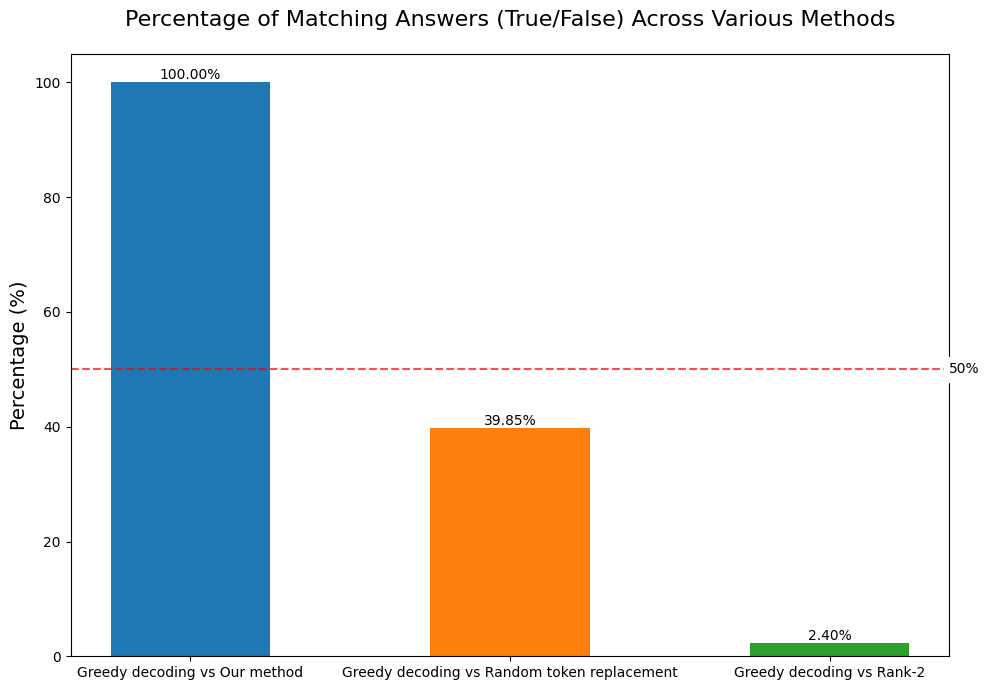
\includegraphics[width=0.8\textwidth]{token_comparison_percentages.png}
\caption{Comparison of decoding methods: Our method achieves higher accuracy in recovering hidden computations compared to random token replacement}
\label{fig:token_comparison}
\end{figure}

\subsection{Discussion}

Our findings indicate that the model internally performs the necessary computations for the 3SUM task and that these computations can be recovered by examining lower-ranked tokens during decoding. The model appears to perform the reasoning in the earlier layers and then overwrites the intermediate representations with filler tokens in the later layers to produce the expected output format.

This overwriting behavior may involve mechanisms such as induction heads \cite{elhage2021mathematical}, where the model learns to copy or overwrite tokens based on patterns in the data. Understanding how the model manages the trade-off between performing computations and producing the expected output could provide valuable insights into the internal workings of transformer models.

Our analysis contributes to the broader understanding of model interpretability and highlights the importance of examining internal representations to gain insights into how models process and represent information. By uncovering the hidden computations, we can develop methods to better control and interpret the outputs of language models, which is crucial for applications where explainability and trust are critical.

\textbf{Limitations:} One limitation of our study is that it focuses on a synthetic task (3SUM) and a relatively small transformer model. While this allows for controlled experimentation, it may not fully capture the complexities of real-world language tasks and larger models. Future work should explore whether similar phenomena occur in larger models and more complex tasks.

\section{Conclusion}

We have presented an analysis of hidden computations in transformer models trained with filler CoT sequences on the 3SUM task. By utilizing the logit lens method and examining token rankings, we demonstrated that the hidden computations can be recovered without loss of performance. Our findings shed light on how models internally process and represent reasoning steps when the explicit chain of thought is obscured.

This work contributes to the broader understanding of model interpretability and opens avenues for improving transparency in language model reasoning. By uncovering the hidden computations, we can gain insights into the internal mechanisms of transformer models and develop methods to better control and interpret their outputs.

\section{Future Work}

Future research should focus on exploring the mechanisms responsible for overwriting the hidden computations with filler tokens. Investigating whether specific circuits, such as induction heads or particular attention patterns, are involved could enhance our understanding of how models balance computation and output formatting.

Moreover, applying similar analysis techniques to other tasks and models could assess the generality of our findings. Extending the investigation to natural language tasks and larger models would help determine whether the observed phenomena persist in more complex settings.

Further work could also explore methods to prevent the overwriting of reasoning steps, allowing models to produce explicit chains of thought even when trained with filler tokens. Developing techniques to enhance the transparency and interpretability of models without compromising performance is an important direction for future research.

\newpage
\appendix

\section{Layer-wise View of Sequences Generated via Various Decoding Methods}

In this appendix, we provide visualizations of the sequences generated using different decoding methods to illustrate how the hidden computations can be recovered.

\begin{figure}[H]
    \centering
    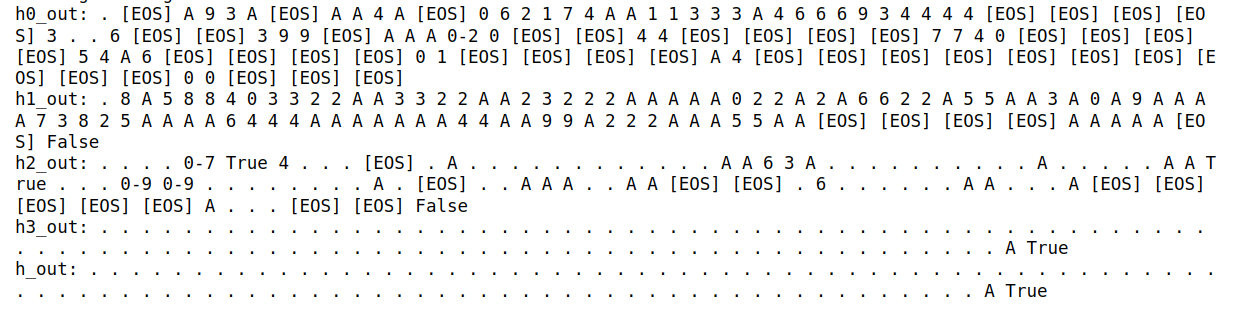
\includegraphics[width=\textwidth]{greedy_decoding.png}
    \caption{Greedy Decoding: The model outputs filler tokens followed by the final answer}
    \label{fig:greedy}
\end{figure}

\begin{figure}[H]
    \centering
    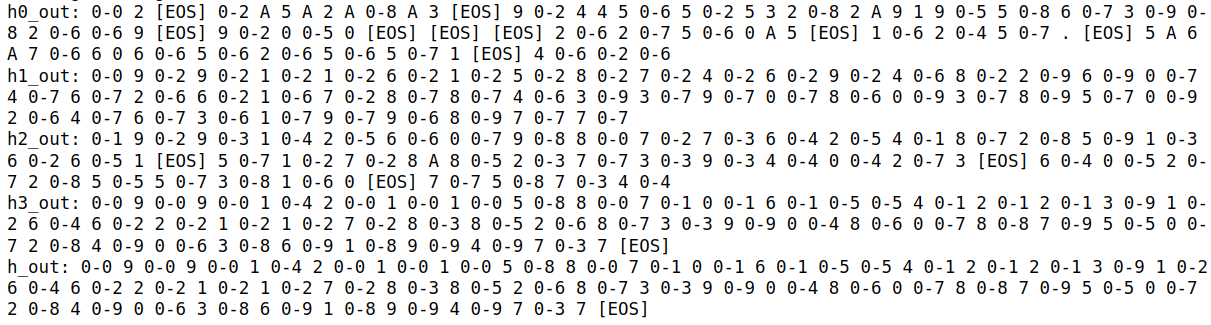
\includegraphics[width=\textwidth]{rank2_decoding.png}
    \caption{Greedy Decoding with Rank-2 Tokens}
    \label{fig:rank2}
\end{figure}

\begin{figure}[H]
    \centering
    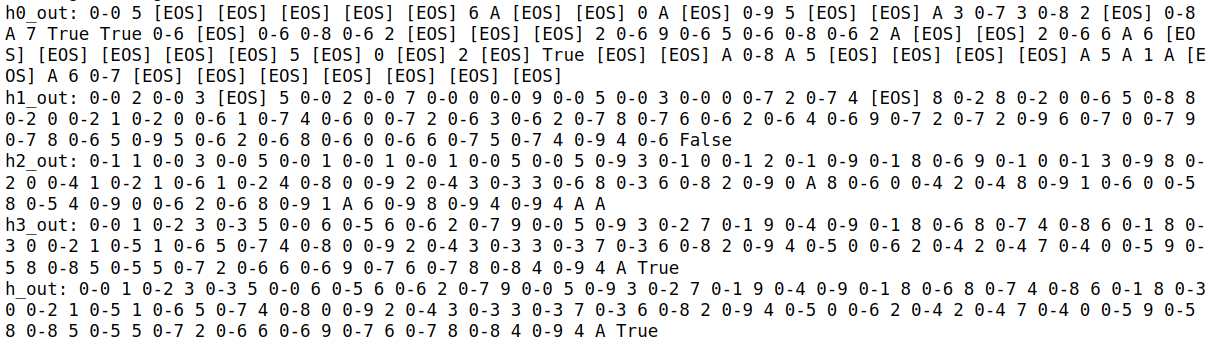
\includegraphics[width=\textwidth]{our_method_decoding.png}
    \caption{Our Method: Greedy Decoding with Filler Tokens Replaced by Lower-Ranked Tokens (Recovering Hidden Computations)}
    \label{fig:our-method}
\end{figure}

\begin{figure}[H]
    \centering
    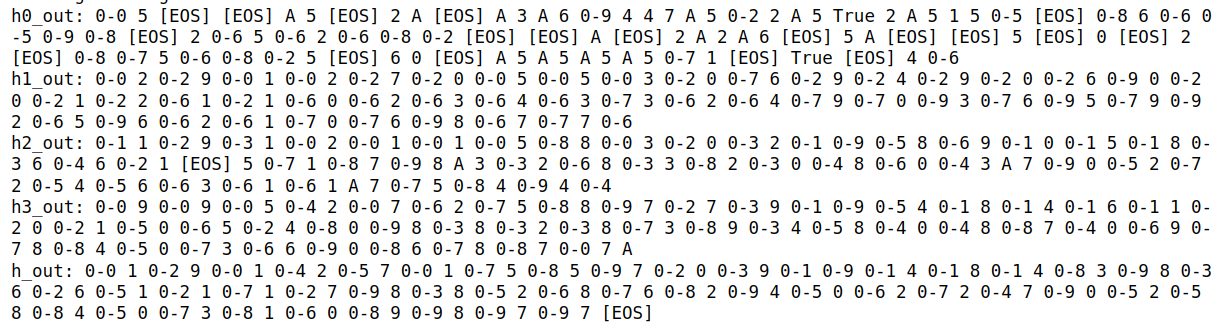
\includegraphics[width=\textwidth]{random_tokens_decoding.png}
    \caption{Random Token Replacement: Replacing Filler Tokens with Random Tokens}
    \label{fig:random}
\end{figure}

As shown in Figures \ref{fig:our-method} and \ref{fig:random}, our method successfully recovers the hidden computations, while random token replacement leads to incoherent sequences.

\newpage
\begin{thebibliography}{9}

\bibitem{wei2022chain}
Jason Wei, Xuezhi Wang, Dale Schuurmans, Maarten Bosma, Brian Ichter, Fei Xia,
  Ed Chi, Quoc Le, and Denny Zhou.
\newblock Chain-of-thought prompting elicits reasoning in large language
  models.
\newblock {\em arXiv preprint arXiv:2201.11903}, 2022.

\bibitem{pfau2023let}
Jacob Pfau, William Merrill, and Samuel~R. Bowman.
\newblock Let's think dot by dot: Hidden computation in transformer language
  models.
\newblock {\em arXiv preprint arXiv:2308.07317}, 2023.

\bibitem{nostalgebraist2020}
Nostalgebraist.
\newblock Interpreting {GPT}: the logit lens.
\newblock
  \url{https://www.lesswrong.com/posts/AcKRB8wDpdaN6v6ru/interpreting-gpt-the-logit-lens},
  2020.

\bibitem{elhage2021mathematical}
Nelson Elhage, Neel Nanda, Catherine Olsson, Nicholas Schiefer, Skyler Hallinan,
  Stanislav Fort, Danny Hernandez, and Chris Olah.
\newblock A mathematical framework for transformer circuits.
\newblock
  \url{https://transformer-circuits.pub/2021/framework/index.html}, 2021.

\bibitem{gao2023shapley}
Xiaoyu Gao.
\newblock Shapley values for interpretability in transformer models.
\newblock {\em arXiv preprint arXiv:2302.00093}, 2023.

\bibitem{madaan2022text}
Divyansh Madaan and Marzieh Yazdanbakhsh.
\newblock Text perturbations for evaluating chain-of-thought reasoning in
  language models.
\newblock {\em arXiv preprint arXiv:2212.08686}, 2022.

\bibitem{turpin2023language}
Jonathan Turpin, Uma Roy, Gabriel Poesia, Jared Kaplan, and Noah Goodman.
\newblock Language models are problem solvers: Formulation of prompts and the
  faithfulness of model reasoning.
\newblock {\em arXiv preprint arXiv:2305.14325}, 2023.

\bibitem{touvron2023llama}
Hugo Touvron, Thibaut Lavril, Gautier Izacard, Edouard Grave, Matthieu
  Lin, Pierre~H. Bluck, Azhar Golriz, Morgan Funtowicz, Lucas
  Sbarra, Aurelien Rodriguez, et~al.
\newblock {LLaMA}: Open and efficient foundation language models.
\newblock {\em arXiv preprint arXiv:2302.13971}, 2023.

\end{thebibliography}

\end{document}

